\section{Method}
\label{sec:method}



\subsection{LLM-Guided Knowledge Graph Traversal with Node Exploration and Exploitation}
\label{sec::llm-guided-traversal}




\begin{wrapfigure}{r}{0.48\textwidth}
\begin{minipage}{\linewidth} 
    \begin{algorithm}[H]
    
    \caption{LLM-Guided KG Traversal}
    \begin{algorithmic}[1]
    \STATE \textbf{Input}: Query $q$, KG $G$, Seed Count $k$, LLM
    \STATE // \textit{Subgraph Initialization}
    \STATE $S \gets$ \text{top-$k$ nodes in $G$ by similarity to $q$}
    \vspace{1mm}
    \STATE // \textit{Path Expansion Loop}
    \REPEAT
    \STATE // \textit{Node Exploration}
    \STATE $a \gets$ \text{LLM selects most answer-relevant } \\ \text{node $a\in S$ }
    \STATE // \textit{Node Exploitation}
    \STATE $S_a \gets \{p \mid edge (a,p) \in G, p \notin S\}$
    \STATE $p \gets$ \text{LLM chooses optimal expansion} \\ \text{node $p\in S_a$ } 
    \STATE $S \gets S \cup \{p\}$
    \STATE $S \gets S \cup \{(a,p)\}$
    \UNTIL{LLM confirms answer is in $S$}
    \STATE \textbf{Output}: $S$
    \end{algorithmic}
    \label{ag:llm-guided-traversal}
    \end{algorithm}
\end{minipage}
\end{wrapfigure}
\textbf{KG Construction}. Building on prior works \cite{Main2,Main6}, we begin by partitioning unstructured text into discrete chunks. Subsequently, we extract named entity triples from these chunks and construct a heterogeneous knowledge graph. This graph comprises two node types: entities and chunks. It also contains two edge types: \textit{entity-chunk edges} (i.e., entity-to-its-source-chunk) and \textit{entity-entity edges} (extracted triples). For specific details on knowledge graph construction, please refer to \Cref{appendix:kg-details}.

\textbf{Graph Traversal}. As illustrated in \Cref{fig:llm-guided-traversal}, \ours~first identifies a set of entity nodes in the knowledge graph that exhibit the highest semantic relevance to the query based on embedding similarity, marking them as \textit{seed nodes}. These seed nodes further form the initial subgraph $S$, which begins with no edges between them. To facilitate effective graph traversal that balances both exploration and exploitation, \ours~iteratively executes two key operations for traversal path expansion: Node Exploration and Node Exploitation. The iteration continues until the LLM determines that subgraph $S$ contains sufficient information to address the query. Refer to \Cref{ag:llm-guided-traversal} and \Cref{appendix:llm-traversal} for details.

\begin{figure}[t]
    \centering
    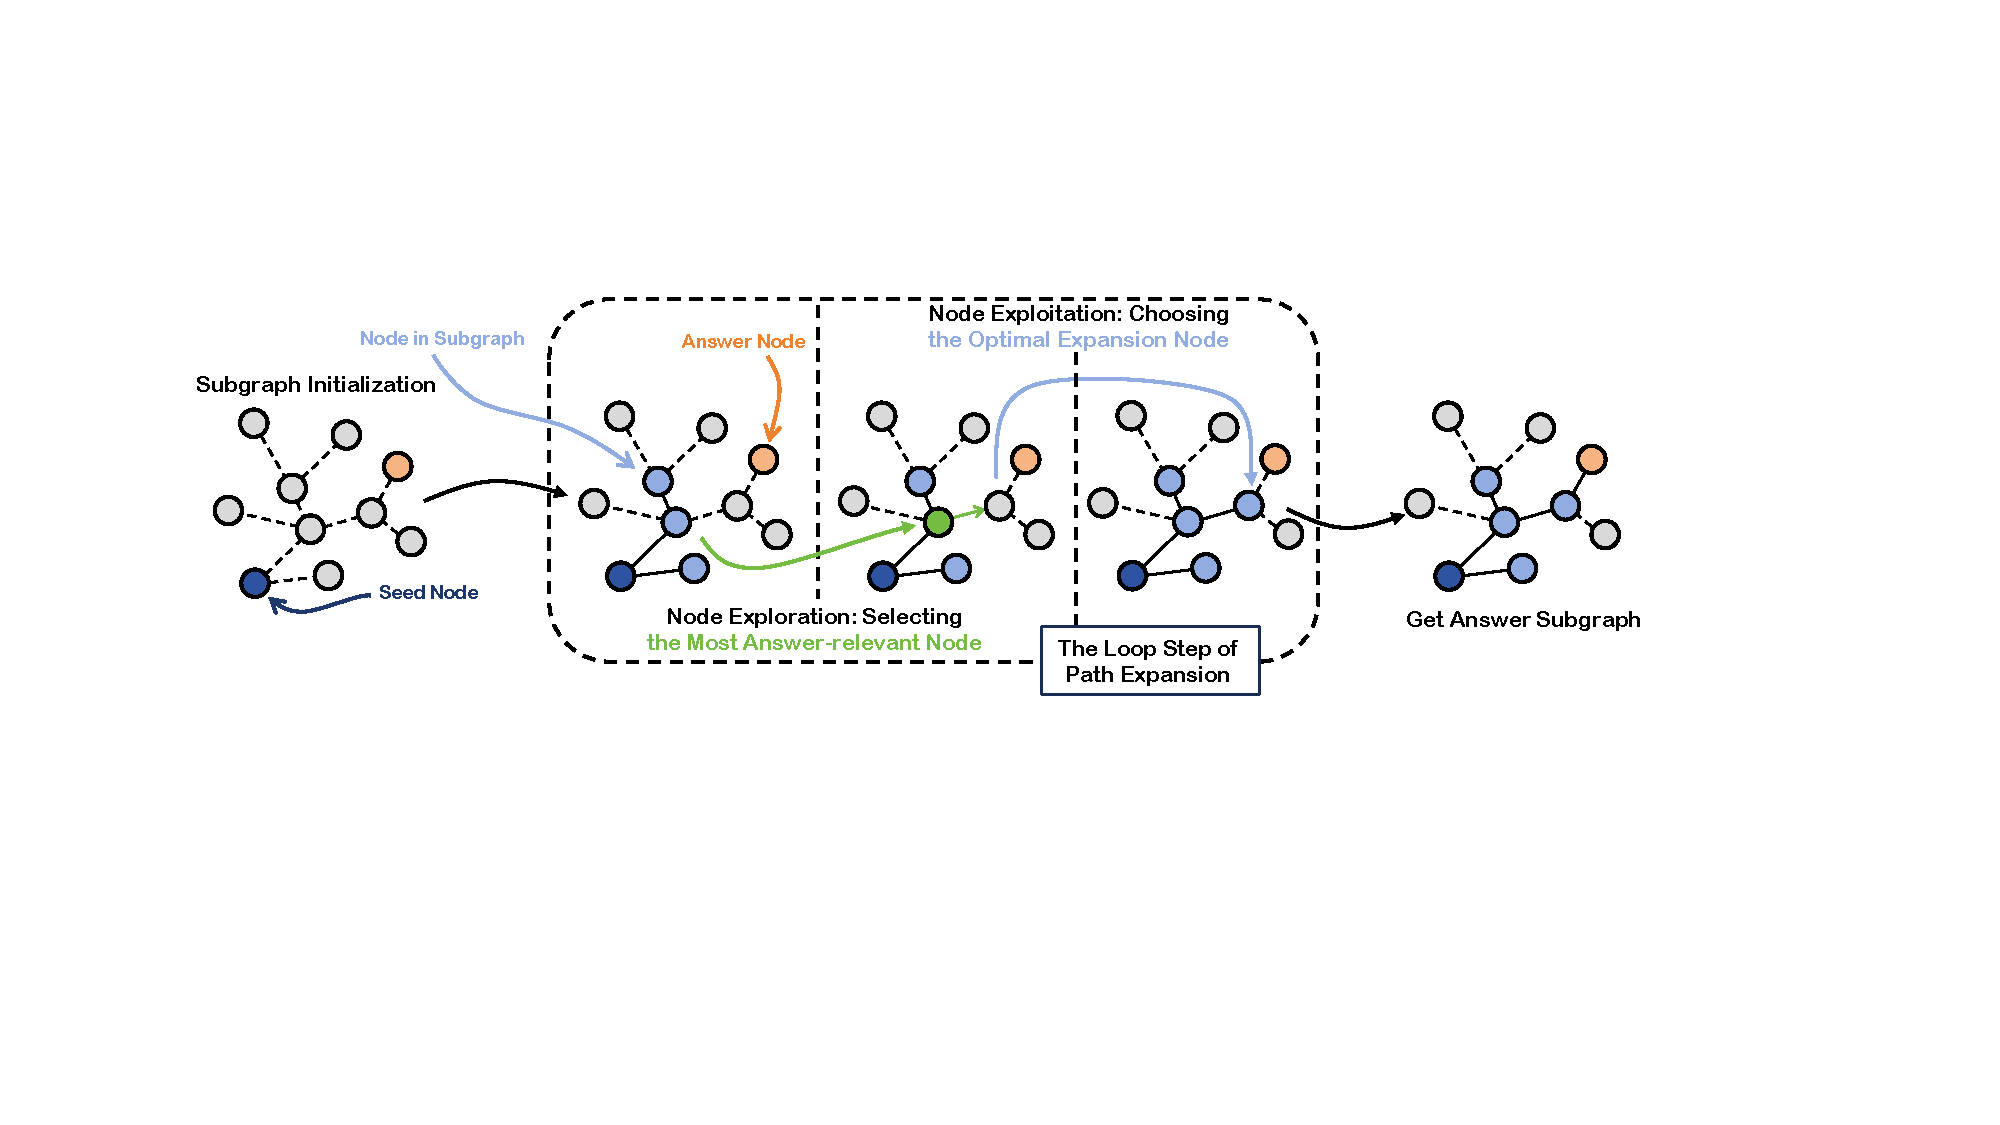
\includegraphics[width=\textwidth]{Resources/LLM-Guide_Traverse.pdf}
    \caption{Illustration of LLM-Guided KG traversal in \ours. It iteratively expands the subgraph towards answer nodes through a process that combines node exploration and exploitation.}
    \label{fig:llm-guided-traversal}
\end{figure}


\begin{itemize}[leftmargin=*]
    \item \textbf{Node Exploration Strategy}. This strategy prioritizes exploring potential nodes likely to lead to the answer, ensuring the graph traversal process is not confined to deep exploration of a single path. Instead, it achieves globally optimal search over the entire KG at low computational cost, thereby increasing the likelihood of obtaining the global optimal solution. To achieve this, during each iteration, the LLM evaluates all nodes in subgraph $S$ and selects the target node $a \in S$ deemed most likely to lead to the answer. 
    
    \item \textbf{Node Exploitation}. This focuses on exploiting previously explored nodes and expanding the path along those nodes to approach the answer. Specifically, given the previously selected node $a \in S$, the LLM selects the optimal expansion node $p$ from the adjacent node set $S_a$ of node $a$, considering $p$ to be the most likely to lead to the answer. At the end of the current iteration, the expansion node $p$ and its connecting path to $a$ are added to subgraph $S$ for subsequent traversal. This leverages the LLM's semantic understanding and reasoning capabilities for effective graph traversal.
\end{itemize}







\subsection{Memory Replay for Efficient Graph Traversal}
\label{sec::traversal-memorizing}
Following previous works regarding memory replay \cite{liu2018effects, wangmemory}, which refers to the recall of valuable past memories to facilitate current tasks, we design memory replay for efficient graph traversal. However, our approach diverges from prior work that typically involves recalling explicit samples. Instead, our `memory' is embedded as weights within the KG, and it is these weights that are exclusively utilized to guide LLM inference and graph traversal. In particular, we design \ours~to memorize LLM's traversal experience within the KG. Consequently, when processing identical, similar and subtly different queries, this memorized experience can be recalled before the LLM-Guided KG Traversal process, reducing the number of LLM calls and significantly enhancing the efficiency while maintaining system effectiveness.


\subsubsection{Memorizing the Traversal Experience within the KG}

\textbf{What to Memorize}. In our work, both effective traversal paths, which lead to the correct answer, and ineffective paths are valuable, as they can provide positive and negative reinforcement, respectively, to guide the LLM's future traversal decisions. Given that the final subgraph $S$ contains a mix of both, we employ a filtering operation: For effective paths, we first use the LLM to identify the edges and chunks that contributed to generating the answer\footnote{We do not provide the ground truth answer to the LLM during this process. The answer here is the one produced by the LLM itself.}, and then use a Depth-First Search (DFS) \cite{dfs} algorithm to extract these paths. The remaining paths are then classified as ineffective.

\begin{equation}
    \begin{aligned}
        \text{\textit{Weight Function}: } \delta(\bm{x}) &= \frac{2}{\pi}\cos\left(\frac{\pi}{2} \|\bm{x}\|_2\right) \\
        \text{\textit{Enhance Effective Path}: } \hat{\bm{v}} &= \bm{v} + \delta(\bm{v}) \cdot \frac{\bm{q}}{\|\bm{q}\|_2} \\
        \text{\textit{Penalize Ineffective Path}: } \hat{\bm{v}} &= \bm{v} - \delta(\frac{\bm{v} \cdot \bm{q}}{\|\bm{q}\|_2}) \cdot \frac{\bm{v} \cdot \bm{q}}{\|\bm{q}\|_2}
    \end{aligned}
\label{eq:update-function}
\end{equation}


\textbf{How to Memorize}. We propose a train-free memorization method to further improve efficiency. This is achieved by memorizing traversal experiences within the KG, which are formalized as edge embeddings and updated using closed-form equations. In particular, after the LLM produces an answer for a query, we update the edge embedding for each edge in the final subgraph $S$\footnote{Each edge in KG has an associated embedding vector, which is subject to updating if that edge is included in the final subgraph.}. Formally, let $v \in R^K$ denote the edge embedding, initialized as a zero vector, where $K$ is the vector dimension. For edges belonging to effective paths within $S$, we update $v$ in the direction of the query embedding $q$ generated by the LLM. Conversely, for edges belonging to ineffective paths, we reduce the component of $v$ along the query embedding $q$ (As shown in \Cref{fig:update-fig}). \Cref{eq:update-function} details the update rules, where $\hat{v}$ represents the updated edge embedding and $\delta$ is the update weight function, which is essentially a cosine function based on the vector's norm.

\begin{figure}[htbp]
    \centering
    \begin{minipage}{0.48\textwidth}
        \centering
        \vphantom{\rule{0pt}{0.7cm}}
        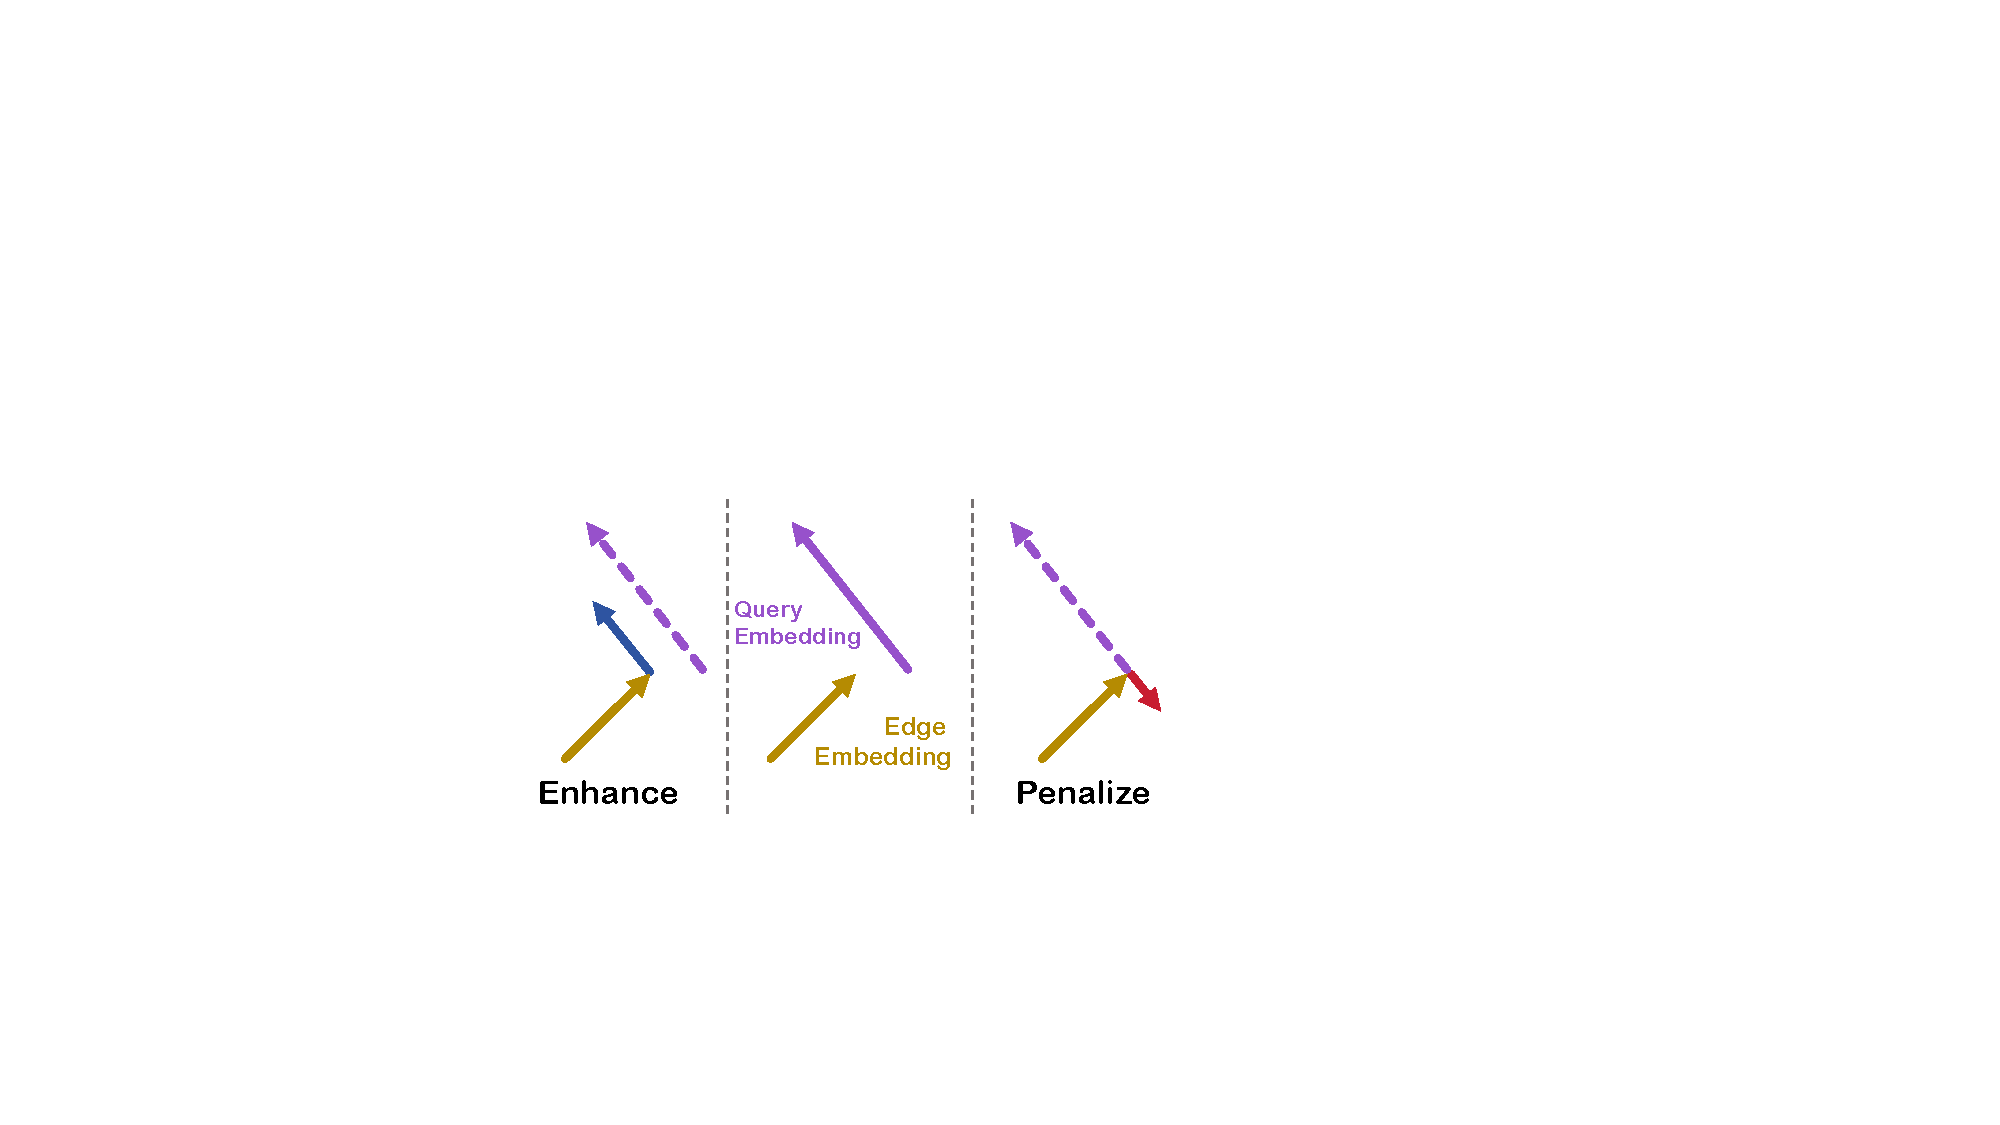
\includegraphics[width=\linewidth]{Resources/embedding_update.pdf}
        \vphantom{\rule{0pt}{0.7cm}}
        \caption{Schematic Diagram of Memorizing.}
        \label{fig:update-fig}
    \end{minipage}
    \hfill
    \begin{minipage}{0.48\textwidth}
        \centering
        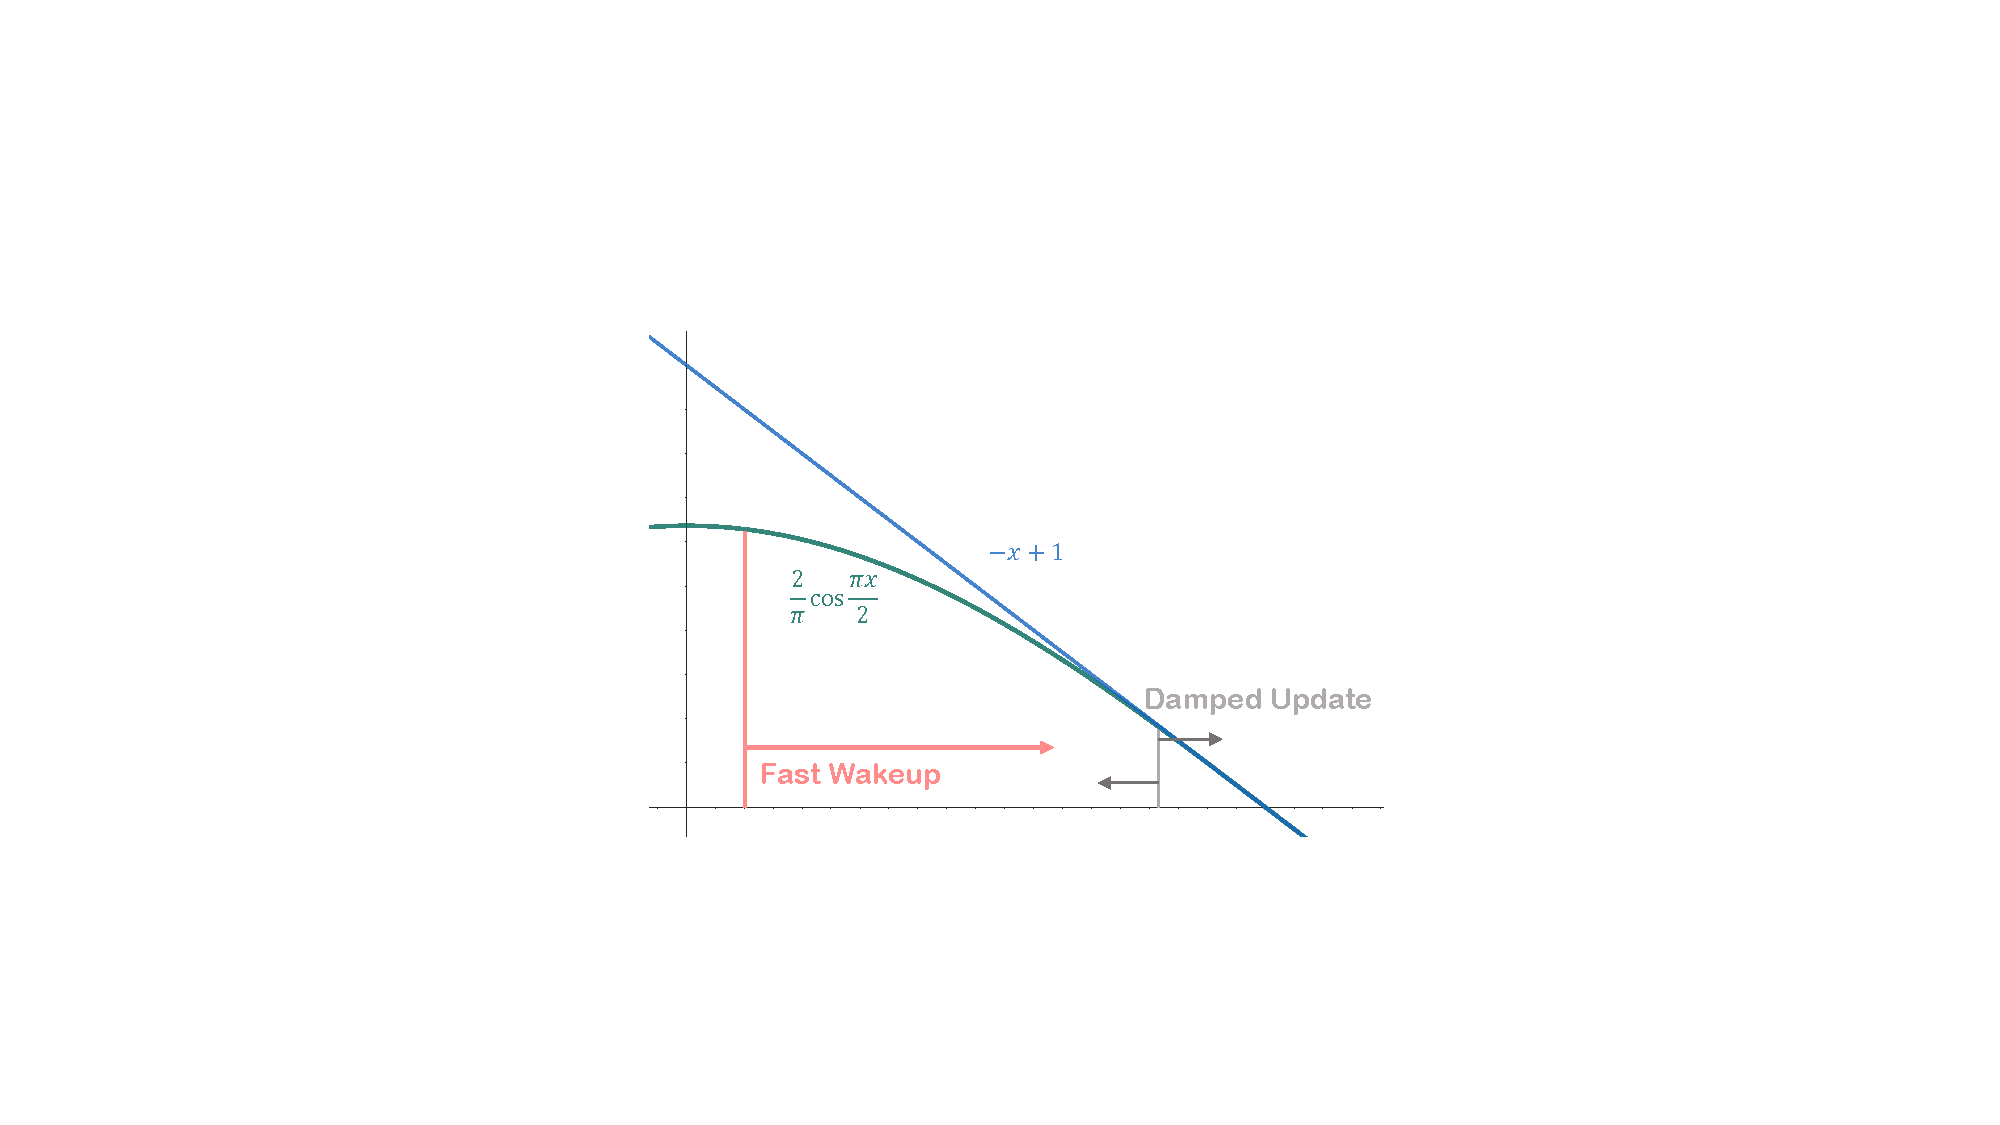
\includegraphics[width=\linewidth]{Resources/theta_function.pdf}
        \caption{Understanding Fast Wakeup \& Damped Update via weight function $\delta$.}  
        \label{fig:delta-fig}
    \end{minipage}
\end{figure}

\textbf{Intuitions Behind Memorizing Process}. Our closed-form memorization rules, as outlined in \Cref{eq:update-function}, exhibit two key characteristics: rapid learning of traversal experiences and sustained stability across multiple memorization events. These characteristics are achieved through the \textit{Fast Wakeup} and \textit{Damped Update}, respectively.
\begin{itemize}[leftmargin=*]
    \item \uline{Fast Wakeup}. When the norm of the edge embedding $v$ is small (typically in the initial all-zero state), it indicates that $v$ retains little memorized information. In this state, we aim for the edge embedding to rapidly learn the traversal experience with only a few updates. As shown in \Cref{fig:delta-fig}, when the norm is small, the $\delta$ function induces a substantial directional update to the edge embedding, thus enabling Fast Wakeup.
    \item \uline{Damped Update.} Once the edge embedding $v$ has learned substantial information (i.e., the norm of $v$ is large), our objective is to maintain the stability of the edge embedding, preventing it from easily losing its learned information due to subsequent updates. As illustrated in \Cref{fig:delta-fig}, the $\delta$ function induces only minor updates when the norm is large, exhibiting resistance to change while retaining the ability to correct errors through gradual forgetting.
\end{itemize}



\subsubsection{Efficient Subgraph Expansion via Memory Replay}
\label{sec::memory-replay}

To enhance traversal efficiency, the memory replay mechanism enriches the initial subgraph $S$ prior to the LLM-guided path expansion (detailed in \Cref{ag:llm-guided-traversal}). This mechanism achieves rapid subgraph expansion by incorporating potentially relevant nodes and edges from historical traversal experiences, thereby reducing reliance on iterative LLM calls.

Formally, let $q$ represent a user query and $G$ denote a knowledge graph, where each edge $E_{ab}$ connecting nodes $a$ and $b$ possesses an associated, updatable embedding vector $v_{ab}$. We define $\text{emb}(\cdot)$ as the text embedding function and $\text{sim}(\cdot, \cdot)$ as the node embedding similarity function. The Subgraph Initialization, detailed in \Cref{ag:llm-guided-traversal}, begins by generating a graph comprising only seed nodes. From each seed node, a recursive Depth-First Search (DFS) is performed to expand the subgraph by adding traversed nodes and edges. This DFS operation proceeds as follows: For a given current node $N_{\text{from}}$ and its unvisited neighbor $N_{\text{to}}$, the system assesses $N_{\text{to}}$'s relevance to both $N_{\text{from}}$ and the query $q$, estimating its potential contribution to the final answer. If this relevance surpasses a predefined threshold $\lambda$, $N_{\text{to}}$ and its connecting edge are incorporated into subgraph $S$, and the DFS process is recursively invoked on $N_{\text{to}}$. The relevance metric $w_{N_{\text{from}},N_{\text{to}}}$, as defined in this work, consists of two components: (1) the semantic relevance between nodes $N_{\text{from}}$ and $N_{\text{to}}$\footnote{This component enables user control over \ours's memory sensitivity.}; and (2) the alignment of traversing the edge with satisfying query $q$, which constitutes \ours's core memory function. The hyperparameter $\alpha$ adjusts the relative importance of these two terms.


\begin{equation}
    w_{N_{from},N_{to}} = \alpha \cdot \mathrm{sim}\big(\mathrm{emb}(N_{from}), \mathrm{emb}(N_{to})\big) + (1-\alpha) \cdot \frac{\mathrm{emb}(q) \cdot v_{N_{from},N_{to}}}{\|\mathrm{emb}(q)\|}
\label{eq:dfs-step-in}
\end{equation}


After subgraph expansion via memory replay, the subgraph is expected to contain sufficient information for answering the input query. However, if the LLM judges that the expanded subgraph still lacks sufficient information, \ours~continues the Path Expansion Loop, a process that can be regarded as verifying and correcting memorized information.
